\documentclass[a4paper, 11pt]{llncs}
\usepackage[top=0.85in, bottom=0.85in, left=0.85in, right=0.85in]{geometry}

%%%%%%%%%%%%%%%%%%%%%%%%%%%%%%%%%%%%%%%%%%%%%%%%%%%%%%%%%%%%%%%%%%%%%%%%%%%%%%%%%%%%%%%%%%
%% Packages
%%%%%%%%%%%%%%%%%%%%%%%%%%%%%%%%%%%%%%%%%%%%%%%%%%%%%%%%%%%%%%%%%%%%%%%%%%%%%%%%%%%%%%%%%%
\usepackage{amsmath}
\usepackage{amsfonts}
\usepackage{amsthm}
\usepackage{graphicx}
\usepackage{xspace}
\usepackage{wrapfig}
\usepackage{enumerate}
\usepackage{cite}
\usepackage{pat}
\usepackage{paralist}
\usepackage{hyperref}
\usepackage{algorithm}
\usepackage{subfig}
%\usepackage{subfigure}
\usepackage{array}
\usepackage[noend]{algpseudocode}
\usepackage[usenames]{xcolor}
\usepackage{stmaryrd} % for lightning-symbol
\usepackage{mathtools} % for mathclap in \conf-definition
\usepackage{todonotes}
%\usepackage{compress}
\usepackage{times}
\usepackage{lineno}

%%\usepackage[font=small,labelfont=bf]{caption}
%\linespread{0.9}
\setlength{\floatsep}{0.9\floatsep}
\setlength{\belowcaptionskip}{2pt}
\setlength{\abovecaptionskip}{4pt}
\setlength{\textfloatsep}{5pt}
\setlength{\intextsep}{5pt}

\let\llncssubparagraph\subparagraph
\let\subparagraph\paragraph
\usepackage{titlesec}
\titlespacing*\section{0pt}{9pt plus 4pt minus 2pt}{3pt plus 2pt minus 0pt}
\titlespacing*\subsection{0pt}{9pt plus 4pt minus 2pt}{3pt plus 2pt minus 0pt}
\titlespacing*\subsubsection{0pt}{9pt plus 4pt minus 2pt}{3pt plus 2pt minus 0pt}


% Save the class definition of \subparagraph
% \let\llncssubparagraph\subparagraph
% Provide a definition to \subparagraph to keep titlesec happy
% \let\subparagraph\paragraph
% Load titlesec
% \usepackage[compact]{titlesec}
% \titlespacing\section{0pt}{6pt plus 4pt minus 2pt}{0pt plus 2pt minus 2pt}
% \titlespacing\subsection{0pt}{6pt plus 4pt minus 2pt}{0pt plus 2pt minus 2pt}
% \titlespacing\subsubsection{0pt}{6pt plus 4pt minus 2pt}{0pt plus 2pt minus 2pt}

\newtheorem{claimx}{Claim}{\bfseries}{\itshape}
%\spnewtheorem{lem}[obs]{Lemma}{\bfseries}{\itshape}
%\spnewtheorem{cor}[theorem]{Corollary}{\bfseries}{\itshape}
%\spnewtheorem{conj}[theorem]{Conjecture}{\bfseries}{\itshape}
%\spnewtheorem{prop}{Property}{\bfseries}{\itshape} % to make property stand out, like lemmata

\newcommand{\false}{\texttt{false}}
\newcommand{\true}{\texttt{true}}
\newcommand{\remove}[1]{}
\newcommand{\red}[1]{\textcolor{red}{#1}}

%% FROM PAT FILE 
\newcommand{\reals}{\mathbb{R}}
\newcommand{\integers}{\mathbb{Z}}
\newcommand{\naturals}{\mathbb{N}}
\newcommand{\dist}{{d}}
\newcommand{\Fary}{F\'ary}


\renewenvironment{proof}
{{\em Proof.\ }}{\hspace*{\fill}$\Box$\par\Vspace{2mm}}

\newenvironment{proofsketch}
{{\em Proof sketch.\ }}{\hspace*{\fill}$\Box$\par\Vspace{2mm}}

\begin{document}
\title{Every Collinear Set Is Free}
\author{Vida Dujmovi\'c\inst{1}\and Fabrizio Frati \inst{2} \and Daniel Gon\c{c}alves \inst{3} \and Pat Morin \inst{4} \and G\"unter Rote\inst{5}}
	\institute{
		University of Ottawa, Canada \hspace{5mm} \email{vida.dujmovic@uottawa.ca} \and 
		Roma Tre University, Italy \hspace{5mm} \email{frati@dia.uniroma3.it} \and
		LIRMM (CNRS \& Universit\'{e} de Montpellier), France \hspace{5mm} \email{daniel.goncalves@lirmm.fr} \and
		Carleton University, Canada \hspace{5mm} \email{morin@scs.carleton.ca}\and
		Freie Universit\"at Berlin, Germany \hspace{5mm} \email{rote@inf.fu-berlin.de}} 
\maketitle

\linenumbers

\begin{abstract}
  We show that if a planar graph $G$ has a plane straight-line embedding
  in which a subset $S$ of its vertices are collinear, then for any
  set of points, $X$, in the plane with $|X|=|S|$ points, there is a plane straight-line
  embedding of $G$ in which the vertices in $S$ are mapped to the points
  in $X$.  This solves an open problem posed by Ravsky and Verbitsky in
  2008.  In their terminology, we show that every collinear set is free.
  
  This result has applications in graph drawing, including untangling,
  column planarity, universal point subsets, and partial simultaneous
  embeddings.
\end{abstract}

\newpage
\pagenumbering{arabic}
\pagestyle{plain}

%!TEX root = mainShort.tex


\section{Introduction}

%A \emph{plane straight-line embedding} of a planar graph $G$ is a
%geometric representation of $G$ where vertices of $G$ are represented
%as a set of points in the plane and each pair of adjacent vertices
%$\{v,w\}$ is connected by a line segment $\overline{vw}$ that
%intersects only $v$ and $w$ and no other edge or vertex in $G$. 

A \emph{straight-line embedding} of a graph $G$ maps each vertex to a point in the plane and each edge to a line segment between its endpoints. A straight-line
embedding is \emph{plane} if no pair of edges cross other than at a
common endpoint. A set
of vertices  $S\subseteq V(G)$ in a planar graph $G$ is a \emph{free
  set} if for any set of points $X$ in the plane with $|X|=|S|$, $G$ has a plane
straight-line embedding in which the vertices of $S$ are mapped to the points in $X$.  Free sets are useful tools in graph drawing
and related areas and have been used to settle problems in untangling~\cite{bose.dujmovic.ea:polynomial,dalozzo.dujmovic.ea:drawing,dujmovic:utility,ravsky.verbitsky:on,ravsky.verbitsky:on-arxiv}, column planarity~\cite{dalozzo.dujmovic.ea:drawing,dujmovic:utility}, universal point subsets~\cite{dalozzo.dujmovic.ea:drawing,dujmovic:utility},
and partial simultaneous geometric embeddings~\cite{dujmovic:utility}.

 A set of vertices  $S\subseteq V(G)$ in a planar graph $G$ is a
 \emph{collinear set} if $G$ has a plane straight-line embedding in
 which all vertices in $S$ are mapped to a single line.  A collinear set $S$
is a \emph{free collinear set} if, for any collinear set of points in
the plane $X$ with $|X|=|S|$, $G$ has a plane straight-line embedding in
which the vertices of $S$ are mapped the points in $X$.  
Ravsky and Verbistky \cite{ravsky.verbitsky:on,ravsky.verbitsky:on-arxiv}
define $\bar{v}(G)$ and $\tilde{v}(G)$ as the respective sizes of the
largest collinear set and largest free collinear set in $G$, and ask
the following question:
%\begin{quote}
	``How far or close are parameters $\tilde{v}(G)$ and $\bar{v}(G)$? It
	seems that \emph{a priori} we even cannot exclude equality. To clarify
	this question, it would be helpful to (dis)prove that every collinear
	set in any straight-line drawing is free.''
%\end{quote}
%
Here, we answer this question by proving that, for every planar graph $G$,
$\tilde{v}(G)=\bar{v}(G)$, that is:

\begin{thm}\thmlabel{our-bang}
Every collinear set is a free collinear set. 
\end{thm}

Let $v(G)$ denote the largest free set for a planar graph $G$. Clearly, we have $v(G)\leq \tilde{v}(G) \leq \bar{v}(G)$. Further, as discussed in detail below, it is well-known that $v(G)=\tilde{v}(G)$. However, prior to our work, the best known bound between $v(G)$,
$\tilde{v}(G)$, and $\bar{v}(G)$ in the other direction was $v(G),\tilde{v}(G) \geq \sqrt{\bar{v}(G)}$, proved by Ravsky and Verbitsky~\cite{ravsky.verbitsky:on}. 
Thanks to \thmref{our-bang}, we now know a stronger bound, in fact the ultimate $v(G)=
\tilde{v}(G) = \bar{v}(G)$ relationship. This relationship was
previously only known for planar $3$-trees
\cite{dalozzo.dujmovic.ea:drawing}. \thmref{our-bang}, in fact, implies a stronger result than $v(G)= \tilde{v}(G) = \bar{v}(G)$:


%Ravsky and Verbitsky
%\cite{ravsky.verbitsky:on} showed earlier that $2$-trees have large, $\Omega(n)$,
%free-colinear sets, however their result did not give
%\thmref{our-bang} for $2$-trees. 




%Before
%\thmref{our-bang}, the following relationships were known between
%$\bar{v}(G)$, $\tilde{v}(G)$ and $v(G)$, starting with the obvious inequality:
%$v(G)\leq \tilde{v}(G) \leq \bar{v}(G)$. It was
%also known that $v(G)=\tilde{v}(G)$, as discussed in detail below. However, in
%the other direction, the best known bound between $v(G)$,
%$\tilde{v}(G)$ and $\bar{v}(G)$ was $\tilde{v}(G) \geq \sqrt{\bar{v}(G)}$ and thus $v(G)\geq
%\sqrt{\bar{v}(G)}$ as proved by Ravsky and Verbitsky~\cite{ravsky.verbitsky:on}.
%%as implied by Theorem 2 in \cite{dujmovic:utility}. 
%This bound, $v(G)\in \Omega(\sqrt{\bar{v}(G)})$, was not strong enough for
%any novel results in the graph drawing applications of free sets. 
%Thanks to \thmref{our-bang}, we now know a much better and more useful bound, in fact the ultimate $v(G)=
%\tilde{v}(G) = \bar{v}(G)$ relationship. This relationship was
%previously only known for planar $3$-trees
%\cite{dalozzo.dujmovic.ea:drawing}. Ravsky and Verbitsky
%\cite{ravsky.verbitsky:on} showed earlier that $2$-trees have large, $\Omega(n)$,
%free-colinear sets, however their result did not give
%\thmref{our-bang} for $2$-trees. 


\begin{cor}\corlabel{our-all}
For every planar graph $G$ and every $S\subseteq V(G)$, $S$ is a free set if
and only if it is a \mbox{collinear set}.
\end{cor}

%\corref{our-all} is a corollary of  \thmref{our-bang} for the
%following reasons. 
That every free set is a collinear set is immediate. \thmref{our-bang} then implies \corref{our-all} since every free collinear set is also a free set. 
This fact, which implies that $v(G)=\tilde{v}(G)$, has been observed by several
authors~\cite{bose.dujmovic.ea:polynomial,dalozzo.dujmovic.ea:drawing,dujmovic:utility,gkossw-upg-09}. To
see this,
let $X=\{(x_1,y_1),\ldots,(x_{|S|},y_{|S|})\}$ and let
$X_0=\{(0,y_1),\ldots,(0,y_{|S|})\}$.  By the definition of free
collinear set, $G$ has a plane straight-line embedding $\Gamma_0$ in
which $S$ maps to $X_0$.  Since the set of plane straight-line embeddings of
$G$ is an open set, there exists some $\epsilon >0$ such that $G$ has a
plane straight-line embedding $\Gamma_{\epsilon}$ in which $S$ maps to
$X_\epsilon=\{(\epsilon x_1,y_1),\ldots,(\epsilon x_{|S|},y_{|S|})\}$.
Dividing all the $x$-coordinates of $\Gamma_\epsilon$ by $\epsilon$ then
yields a plane straight-line embedding $\Gamma$ in which $S$ maps to
$X$. 

Thus, \thmref{our-bang} is our main result and this paper is dedicated to
proving it. The following
characterization of collinear sets by Da Lozzo \etal\
\cite{dalozzo.dujmovic.ea:drawing}  is helpful in that goal.

\begin{thm}\cite{dalozzo.dujmovic.ea:drawing} \thmlabel{collinear-set}
	A set $S$ of the vertices of a graph $G$ is a collinear set if and
	only if there is a plane embedding of $G$ and a Jordan curve $C$
	that contains every vertex in $S$, that intersects the interior of
	at least one face of $G$, and whose intersection with
	each edge of $G$ is either empty, a single point, or the entire edge.
\end{thm}

 \thmref{collinear-set} is helpful because it reduces the problem of
finding large collinear sets in a graph $G$ to a topological game in
which one only needs to find a curve that contains many vertices
of $G$.  Indeed, Da Lozzo \etal\ used \thmref{collinear-set} to give
tight lower bounds on the sizes of collinear sets in planar graphs
of treewidth at most 3 and triconnected cubic planar graphs. Despite the conceptual simplification provided by \thmref{collinear-set},
the identification of collinear sets is highly non-trivial:  Mchedlidze
\etal\ \cite{mchedlidze.radermacher.ea:aligned} showed that it is NP-hard to
determine if a given set of 5 vertices in a planar graph is a collinear
set.
%
Nevertheless, \thmref{collinear-set} is a useful tool for finding large 
collinear sets. This in combination with \corref{our-all} gives a useful
tool for finding free sets, which have a wide variety of applications,
as outlined in the next section.


\subsection{Applications and Related Work}

The applicability of \corref{our-all} comes from the fact that a number of graph drawing applications require (large) free sets, whereas finding large collinear sets
is an easier task. Indeed there are planar graphs for which large collinear sets were known to exist, however large free sets were not. Those include 3-connected cubic planar graphs
and planar graphs of treewidth at least $k$.
%
%Free collinear sets have a number of applications in graph drawing and related areas. 
%We now review applications of our result. 

%A \emph{geometric graph} is a graph $G$ whose vertices are distinct
%points in the plane (not necessarily in general position) and whose
%edges are straight-line segments between pairs of points.  If the
%underlying combinatorial graph of $G$ belongs to a class of graphs
%$\mathcal K$, then we say that $G$ is a \emph{geometric $\mathcal K$ graph}. 

%\paragraph{Untangling} \cite{bose.dujmovic.ea:polynomial,cano.toth.ea:upper,c-upg-10,dalozzo.dujmovic.ea:drawing,dujmovic:utility,gkossw-upg-09,kpr-upg-11,pt-up-02,ravsky.verbitsky:on,ravsky.verbitsky:on-arxiv}

\paragraph{Untangling.}  Given a straight-line embedding of a planar
graph $G$, possibly with crossings, to \emph{untangle} it means to assign
new locations to some of the vertices of $G$ so that the resulting
straight-line embedding of $G$ is plane. The goal is to do so while
\emph{keeping fixed} (that is, while not changing the location of) as many vertices as possible. In 1998 Watanabe asked if every polygon can be untangled while keeping at least $\varepsilon n$ vertices
fixed, for some $\varepsilon >0$ . Pach and Tardos\cite{pt-up-02} answered that question in
the negative by providing an $\mathcal{O}((n\log n)^{2/3})$ upper bound on the
number of fixed vertices. This has almost been  matched by
an 
$\Omega(n^{2/3})$ lower bound by Cibulka~\cite{c-upg-10}. Several papers have studied the untangling
problem~\cite{pt-up-02,cano.toth.ea:upper,c-upg-10,bose.dujmovic.ea:polynomial,gkossw-upg-09, kpr-upg-11,ravsky.verbitsky:on}. Asymptotically tight
bounds are known for paths \cite{c-upg-10}, trees \cite{gkossw-upg-09}, outerplanar graphs
\cite{gkossw-upg-09}, and planar graphs of treewidth two and three \cite{ravsky.verbitsky:on,
  dalozzo.dujmovic.ea:drawing}. For general
planar graphs there is still a large gap. Namely, it is known that every planar graph can be untangled while
keeping $\Omega(n^{0.25})$ vertices fixed
\cite{bose.dujmovic.ea:polynomial} (this answered a 
question by Pach and Tardos \cite{pt-up-02})  and that there are planar graphs
that cannot be untangled while keeping $\Omega(n^{0.4948})$ vertices
fixed \cite{cano.toth.ea:upper}. \thmref{our-bang} can help close this gap, whenever a good bound
on collinear sets is known.  %The connection between untangling and
                              %free sets comes from the following. 
Namely, Bose \etal\cite{bose.dujmovic.ea:polynomial} implicitly and  Ravsky and Verbitsky
\cite{ravsky.verbitsky:on} explicitly, proved that every straight-line
embedding of a planar graph $G$ can be untangled while keeping
$\Omega(\sqrt{|S|})$ vertices fixed, where $S$ is a free set of
$G$. Together with \corref{our-all} this implies that, for untangling, it is enough to
find large collinear sets.

\begin{thm}\thmlabel{our-untang}
Let $S$ be a collinear set of $G$. Every straight-line embedding of a
planar graph $G$ can be untangled while keeping $\Omega(\sqrt{|S|})$ vertices fixed.
\end{thm}

Da Lozzo \etal~\cite{dalozzo.dujmovic.ea:drawing}  proved that every 3-connected cubic planar graph has
a $\Omega(n)$ collinear set. Then \thmref{our-untang} implies the
following new result, for which $\Omega(n^{0.25})$ was a previously
  best known \mbox{untangling bound.} 
%  Note that triconnected cubic planar
%graphs form a rich subclass of planar graphs as they are duals of
%(non-trivial) triangulations.

\begin{cor}\corlabel{our-cubic-unt}
A straight-line embedding of every $n$-vertex triconnected cubic
planar graph can be untangled while 
keeping $\Omega(\sqrt{n})$ vertices fixed. 
\end{cor}

This result is almost tight due to the $\mathcal{O}(\sqrt{n\log^3n })$ upper bound for 3-connected cubic planar graphs of diameter $\mathcal{O}(\log n)$ \cite{c-upg-10}. This result cannot be extended to all bounded-degree planar graphs (see \cite{dujmovic:utility,DBLP:journals/dm/Owens81} for
reasons why).  Da Lozzo \etal\ also proved that planar graphs of treewidth at least
$k$ have  have $\Omega(k^2)$-size collinear sets. Together with
\thmref{our-untang}  that implies that 
%
%, the following:
%\begin{cor}\corlabel{our-tw}
every straight-line embedding of an $n$-vertex planar graph of treewidth
at least $k$ can be untangled while keeping $\Omega(k)$ vertices fixed. 
%\end{cor}
%
This gives, for example, a tight $\Theta(\sqrt{n})$
untangling bound for planar graphs of treewidth
$\Theta(\sqrt{n})$.  

Our result have applications beyond untangling. The full version of the paper, available after the bibliography, describes applications to the {\em universal point subset} problem~\cite{abehlmmo-ups-12,dalozzo.dujmovic.ea:drawing,dujmovic:utility}, a problem derived from the notorious {\em universal point set} problem~\cite{DBLP:journals/comgeo/Bose02,DBLP:conf/cccg/CastanedaU96,deFraysseix:1988:SSS:62212.62254, dFPP90, GMPP,DBLP:journals/ipl/Kurowski04, DBLP:journals/jgaa/BannisterCDE14}. Similar applications of \thmref{our-bang} and \corref{our-all} to problems such
as \emph{column planarity}~\cite{behks-cppsge-17,dalozzo.dujmovic.ea:drawing,dujmovic:utility}
and \emph{partial simultaneous geometric embeddings with and without
  mappings}~\cite{behks-cppsge-17,ddlmw-pqp-15,dujmovic:utility} are possible as described in the survey by Dujmovi\'c~\cite{dujmovic:utility}.


% Cano \etal\ \cite[Theorem~2]{cano.toth.ea:upper} show that if a Jordan
% curve $C$ intersects each edge of a plane embedding of a graph $G$ in
% at most one point and does not contain any vertex of $G$, then $G$ has
% a straight-line plane embedding in which the edges of $G$ intersected
% by $C$ become line segments that cross the $y$-axis, and these crossings
% occur in the same order.  A restatement of \thmref{collinear-set} that
% we describe as \thmref{dujmovic-frati} in \secref{definitions} gives an
% extension of this result to curves that include vertices of $G$.

\subsection{Proof Outline for \thmref{our-bang}}

We assume w.l.o.g.\ that $G$ is a plane straight-line
embedded graph in which the collinear set $S\subseteq V(G)$ is embedded
on the $y$-axis $Y=\{(0,y):y\in\R\}$. Let
$L=\{(x,y)\in\R^2:x<0\}$ and $R=\{(x,y)\in\R^2: x >0\}$ denote the open
halfplanes to the left and right of $Y$. When talking about the order of points on the $y$-axis $Y$, we are referring to the total order $\prec_Y$ in which $(0,a) \prec_Y (0,b)$ if and only if $a<b$. We assume, furthermore, that we are given $|S|$ distinct $y$-coordinates and the goal is to find another plane straight-line embedding of $G$ in which the vertices in $S$ are embedded on $Y$ with the given $y$-coordinates.

Tutte's Convex Embedding Theorem \cite{tutte:how} allows one to (plane
straight-line) embed an internally 3-connected graph with the vertices
of the outer face embedded on any prescribed convex polygon with the
correct number of vertices.  If the vertices in $S$ induce a path with
both endvertices on the outer face of $G$, then no edge of $G$ crosses
$Y$. Then it is easy to prove that $S$ is a free
collinear set using two applications of \cite{tutte:how}, on (suitable augmentations of) the graphs induced
by $V(G)\cap(L\cup Y)$ and $V(G)\cap(Y\cup R)$.

Thus, the main difficulty comes from edges of $G$ that cross $Y$.
These edges must be embedded so that they cross $Y$ in prescribed
intervals between the prescribed locations of vertices in $S$, and
these intervals may be arbitrarily small.  An extreme version of this
(sub)problem is the one in which $G$ is an embedded graph where every
edge intersects $Y$ in exactly one point (possibly an endpoint) and
the location of each crossing point is prescribed.  The most difficult
instances occur when $G$ is edge-maximal.

In \secref{quadrangulations} we describe these edge-maximal graphs, which
we call A-graphs.  A-graphs are a generalization of quadrangulations in
which every face is either a quadrangle whose every edge intersects $Y$ or a triangle with one vertex in
each of $L$, $Y$, and $R$.  \thmref{a-graph} in this section shows that it
is possible to find a plane straight-line embedding of any A-graph where
the intersections of the embedding with $Y$ occur at prescribed locations.
This is done by showing that a certain system of linear equations has
a solution. This proof involves some linear algebra and some arguments
that use continuity.

In \secref{triangulations} we prove that every collinear set is free.
The technical statement of this result, \thmref{main}, shows a somewhat
stronger result for triangulations that makes it possible not only to
prescribe the locations of vertices on $Y$ but also to nearly prescribe the
points at which edges of $T$ cross $Y$.  This proof uses combinatorial
reductions that are applied to a triangulation $T$ that either reduce its
size or increase the number of edges that cross $Y$.  When none of these
reductions is applicable to $T$, removing the edges of $T$ that do not
cross $Y$ creates an A-graph, $G$, on which we can apply \thmref{a-graph}.

\secref{definitions}, next, presents preliminary definitions and results. Because of space limitations, several proofs are omitted or sketched. They can be found in the full version of the paper, which follows the bibliography.

%!TEX root = mainShort.tex
\section{Preliminaries}
\seclabel{definitions}

We begin with fairly standard definitions and then move on to problem-specific definitions and results.

%\subsection{Standard Definitions}

For a function $f:\R\to\R$, we use $\lim_{x\downarrow t} f(x)$ and
$\lim_{x\uparrow t} f(x)$ to denote the one-sided limits of $f(x)$
as $x$ approaches $t$ from above and below, respectively.  
%
A \emph{curve} $C$ is a continuous function from $[0,1]$
to $\mathbb{R}^2$.  The points $C(0)$ and $C(1)$ are the \emph{endpoints} of $C$.  A curve $C$ is \emph{simple} if $C(s)\neq C(t)$
for any $0\le s<t< 1$; it is \emph{closed} if $C(0)=C(1)$.  A \emph{Jordan
	curve} $C:[0,1]\to\R^2$ is a simple closed curve.  
%Starting in the current paragraph, 
We will often fail to distinguish between a curve $C$ and its
image $\{C(t):0\le t\le 1\}$.  When this happens, we may qualify the curve as
\emph{open} in which case we are referring to the set $\{C(t):0< t< 1\}$.
A point $x\in\R^2$ is \emph{on} $C$ if $x\in C$.  
%
For any Jordan curve $C$, $\R^2\setminus C$ has two connected
components: One of these, $C^-$, is finite (the {\em interior} of $C$) and the other, $C^+$, is
infinite (the {\em exterior} of $C$).  
%We say that a Jordan curve is \emph{well-oriented} if walking
%along $C$ from $C(0)$ to $C(1)$ results in a counterclockwise traversal
%of the boundary of $C^-$, so that $C^-$ is locally to the left of $C$
%and $C^+$ is locally to the right of $C$. NOT USED?
%
The points on a simple curve $C$ are associated with a partial order $\prec_C$ such that $C(a)\prec_C C(b)$ if and only if $a<b$.  

%For any $0\le a\le b\le 1$, the \emph{subcurve}
%of $C$ between $a$ and $b$ is the curve $C'(t)=C(a+t(b-a))$.  When talking about the subcurve of $C$ between points $x,y\in C$ where $x\prec_C y$, we mean the subcurve of $C$ between the unique $a< b$ with $x=C(a)$ and $y=C(b)$. NOT USED?

All graphs $G$ considered in this paper are finite, simple, and
undirected.   We use $V(G)$ and $E(G)$ to denote the vertex set and edge
set of $G$, respectively. We denote by $d_v$ the degree of a vertex $v$ in a graph. 

An \emph{embedding} $\Gamma=(\varphi,\rho)$ of a graph $G$ consists
of a one-to-one mapping $\varphi:V(G)\to\R^2$ and a mapping $\rho$ from
$E(G)$ to curves in $\R^2$ such that, for each edge $xy\in E(G)$, $\rho(xy)$
has endpoints $\varphi(x)$ and $\varphi(y)$.
%Starting immediately,  
We often say that $G$ is an embedded graph
without explicitly referring to the pair $\Gamma=(\varphi,\rho)$.
In these cases, we identify vertices of $G$ with their
points and edges of $G$ with their curves. By default, an edge curve includes
its endpoints, otherwise we specify that it is an \emph{open} edge.
%
In a \emph{straight-line embedding} each edge is a straight-line segment. In a \emph{plane embedding} no two edges intersect, except possibly at common endpoints. A \emph{F\'ary embedding} is a plane straight-line embedding. For a given F\'ary embedding $G$, we often address the problem of constructing a different F\'ary embedding of $G$, satisfying certain properties; by this we mean that we will construct a F\'ary embedding of the plane embedded graph of which $G$ is a F\'ary embedding.
%
The \emph{faces} of an embedded graph $G$ are the maximal connected
subsets of $\R^2\setminus\bigcup_{xy\in E(G)} xy$.  One of
these faces, the \emph{outer} face, is unbounded; the other faces are called \emph{inner} or \emph{bounded} faces. A {\em boundary vertex} is incident to the outer face, other vertices are called \emph{interior} vertices.
A \emph{triangulation} (a \emph{quadrangulation}) is a plane embedded graph in which each face is bounded by a 3-cycle (respectively, 4-cycle). 
%A \emph{chord} is an edge of $G$ with two endpoints on the outer face but whose
%interior is not on the outer face.  
%When discussing plane embeddings, we use the convention of listing
%the vertices of a face as they appear when traversing the face in
%counterclockwise order. NOT REALLY

%Every quadrangulation has
%$n\ge 4$ vertices and Euler's formula implies that it has $2n-4$ edges. NOT USED?
%A \emph{near-quadrangulation} is a plane embedded graph in which each
%inner face (but not necessarily the outer face) is bounded by a 4-cycle.
%An \emph{outerplanar graph} is a plane embedded graph in which there is
%a single face that is incident to every vertex.

A \emph{separating cycle} of a graph $G$ is a sequence of vertices
that form a cycle and whose removal disconnects $G$.  A \emph{separating triangle} is
a separating cycle of length 3.  
If $G$ is a plane embedded graph, then,
for any separating cycle $C$, there is a 
%well-oriented 
Jordan curve whose image
is the union of edges in $C$.  In this case, the interior and exterior of
$C$ refer to the interior and exterior of the corresponding Jordan curve.

The \emph{contraction} of an edge $xy$ in a graph $G$ identifies $x$ and $y$ to obtain a new graph $G'$ with
$V(G')=V(G)\cup\{v\}\setminus\{x,y\}$ and $E(G')=E(G)\setminus\{ab\in
E(G): \{a,b\}\cap\{x,y\}\neq\emptyset\}\cup\{va: xa\in E(G)\}\cup
\{va:ya\in E(G)\}$.  
%In this case, we say that we \emph{contract} $xy$ in $G$ to obtain the graph $G'$.  EASY TO FIGURE
If $G$ is a triangulation and we
contract the edge $xy\in E(G)$, then the resulting graph $G'$ is also
a triangulation provided that $xy$ is not part of any separating
triangle. More specifically, the plane embedding of $G$ extends naturally
to a plane embedding of $G'$.

%\subsection{Problem Specific Definitions}

A %well-oriented 
Jordan curve $C$ is \emph{admissible} for an
embedded graph $G$ if $C(0)=C(1)$ is in the outer face
of $G$ and the intersection between $C$ and each edge $e$ of $G$ is
either empty, a single point, or the entire edge $e$.  
%We say that $C$
%is \emph{proper} for $G$ if it is admissible and it does not contain any
%vertex of $G$; i.e., $C$ is proper if its intersection with any edge $e$
%of $G$ is either empty, or in the interior of $e$.

%We say that a Jordan curve $C:[0,1]\to\R^2$ is \emph{nice} for an embedded
%graph $G$ if $C$ intersects each edge of $G$ in at most one connected
%component and the endpoint $C(0)=C(1)$ of $C$ is in the interior of the
%outer face of $G$.  We say that $C$ is \emph{clean} (for $G$) if its
%intersection with each edge of $G$ is either empty or a single point.
%We say that $C$ is \emph{tidy} (for $G$) if it does not contain any
%vertex of $G$.

We will make use of the following restatement of \thmref{collinear-set}
which follows from the proof in \cite{dalozzo.dujmovic.ea:drawing}:
\begin{thm}\thmlabel{dujmovic-frati}
	For any planar graph $G$, the following two statements are equivalent: (1) There exists a plane embedding $\Gamma_1$ of $G$ and an admissible curve $C:[0,1]\to\R^2$ such that the sequence of edges and vertices intersected by $C$ is $r_1,\ldots,r_k$. (2) $G$ has a \Fary\ embedding $\Gamma_2$ in which the sequence
		of edges and vertices intersected by $Y$ is $r_1,\ldots,r_k$.
\end{thm}


%!TEX root = mainShort.tex
\section{A-Graphs}
\seclabel{quad}
\seclabel{quadrangulations}

In this section, we study a special class of graphs that are closely
related to quadrangulations in which every edge crosses $Y$. (See \figref{a-graph} for an example.)

\begin{definition}\deflabel{a-graph}
	An \emph{A-graph}, $G$, is a \Fary\ embedding of a graph with $n\ge 3$ vertices that has the following properties: (1) Every edge of $G$ intersects $Y$ in exactly one point, possibly an endpoint. (2) Every face of $G$, including the outer face, is a quadrilateral or a triangle. (3) Every quadrilateral face of $G$ is non-convex. (4) Every triangular face contains one vertex in each of $Y$, $L$, and $R$. (5) Every vertex $v$ on $Y$ is incident to precisely
		two triangular faces, one ``above $v$'' whose interior contains the open line segment with endpoints $v$ and $v+(0,\epsilon)$ for some $\epsilon>0$ and one ``below $v$'' whose interior contains the open line segment with endpoints $v$ and $v-(0,\epsilon)$ for some $\epsilon >0$.
\end{definition}

\begin{wrapfigure}[11]{r}{.3\textwidth}
		\Vspace{-1mm}
		\centering
		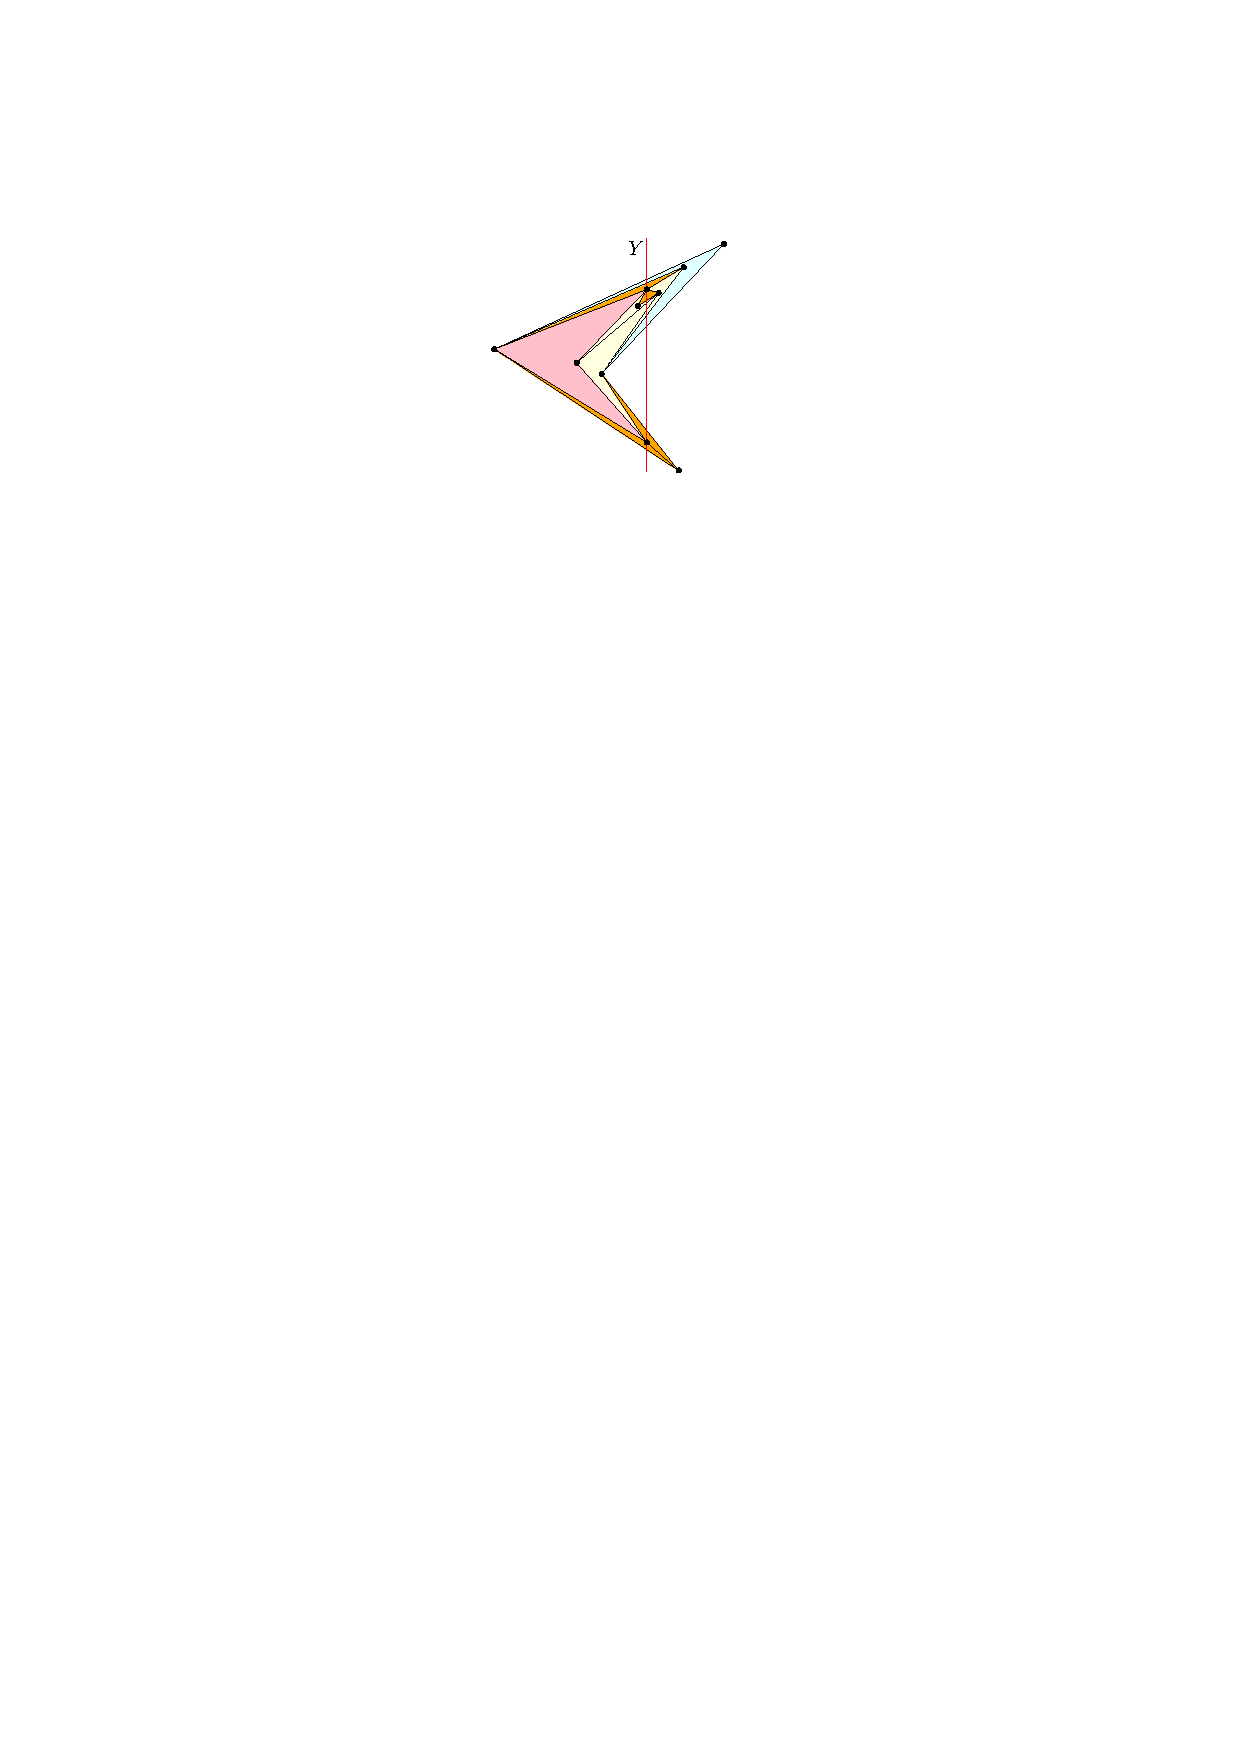
\includegraphics[scale = 0.95]{figs/a-graph-new}
		\caption{An A-graph with 2 vertices in $Y$.}
		\figlabel{a-graph}
	\end{wrapfigure}
	
In the special case where $G$ has no vertices in $Y$, the graph $G$ is a quadrangulation in which every edge crosses $Y$. Further, Property~5 applies even if $v$ is on the outer face of $G$ (in which case it implies that the outer face of $G$ must be a triangle).
Some additional properties of $G$ follow from \defref{a-graph}: (6) $G$ is connected. (7) Every vertex of $G$ has degree at least 2. (8) If $n\ge 4$, then every vertex in $Y$ has degree at least 3.  Property~6 follows directly from Property~2.
Property~7 follows from the fact that every vertex is incident to at
least one face and every face is a simple cycle.
Property~8 follows from the fact that every vertex on $Y$ is incident
to at least two triangular faces, which involve at least 4 vertices, unless $n=3$.

%We will show that every A-graph $G$ has a \Fary\ embedding with prescribed
%intersections with $Y$ and a prescribed outer face.  Since the outer
%face of an A-graph can be a triangle or a quadrilateral, in the following
%theorem, $\Delta$ is a triangle or quadrilateral defined as follows:
%\begin{enumerate}
%   \item If $(0,y_1)$ is a vertex of $G$, then $\Delta$ is a triangle
%   with one vertex at $(0,y_1)$ and the opposite edge edge crossing $Y$ at $y_m$.
%
%   \item If $(0,y_m)$ is a vertex of $G$, then $\Delta$ is a triangle
%   with one vertex at $(0,y_m)$ and the opposite edge crossing $Y$ at $y_1$.
%
%   \item Otherwise,
%      $\Delta$ is a quadrilateral whose edges cross $Y$ at $y_1$, $y_a$,
%      $y_b$, and $y_m$, where $e_1$, $e_a$, $e_b$, and $e_m$ are the four edges on the outer face of $G$
%\end{enumerate}

We will show that every A-graph $G$ has a \Fary\ embedding with prescribed intersections with $Y$ and a prescribed outer face, as in the following theorem. 

\begin{thm}\thmlabel{a-graph}
	Let $G$ be an A-graph, let $e_1,\ldots,e_m$ be the sequence of edges in $G$, in the order they are intersected by $Y$, and let $y_1\le\cdots\le y_m$ be any sequence of numbers where, for each $i\in\{1,\ldots,m-1\}$, $y_i=y_{i+1}$ if and only if $e_i$ and $e_{i+1}$ have a common endpoint in $Y$. Further, let $\Delta$ \mbox{be a triangle or quadrilateral, where:}
		\begin{compactenum}
			\item If $(0,y_1)$ is a vertex of $G$, then $\Delta$ is a triangle
			with a vertex at $(0,y_1)$ and the opposite edge crossing $Y$ at $y_m$.
			
			\item If $(0,y_m)$ is a vertex of $G$, then $\Delta$ is a triangle
			with a vertex at $(0,y_m)$ and the opposite edge crossing $Y$ at $y_1$.
			
			\item Otherwise, $\Delta$ is a quadrilateral whose edges cross $Y$ at $y_1$, $y_a$,
			$y_b$, and $y_m$, where $e_1$, $e_a$, $e_b$, and $e_m$ are the four edges on the outer face of $G$.
	\end{compactenum}
	Then $G$ has a
	\Fary\ embedding in which the outer face is $\Delta$
	and, for each $i\in\{1,\ldots,m\}$, the intersection between $e_i$ and $Y$
	is the single point $(0,y_i)$.
\end{thm}

The rest of this section is devoted to prove \thmref{a-graph}. We make some simplifying assumptions. First, we assume w.l.o.g.\ up to a uniform scaling that $\Delta$ and all the vertices of $G$ are contained in $[-1,1]^2$. Second, we assume w.l.o.g.\ up to a reflection  with respect to $Y$ that, if the outer face of $G$ is delimited by a quadrilateral, then the vertex incident to both $e_1$ and $e_m$ is in $L$, as in \figref{a-graph}. In such a case we also assume that the vertex of $\Delta$ incident to both $e_1$ and $e_m$ is in $L$; this is also not a loss of generality, as if the vertex of $\Delta$ incident to both $e_1$ and $e_m$ is in $R$, then $\Delta$ can be reflected with respect to $Y$, obtaining a quadrilateral $\Delta'$ whose vertex incident to both $e_1$ and $e_m$ is in $L$, then a \Fary\ embedding of $G$ can be constructed in which the outer face is $\Delta'$, and finally the \Fary\ embedding can be reflected with respect to $Y$, thus obtaining a \Fary\ embedding of $G$ in which the outer face is $\Delta$. 

If $m=3$ or $m=4$, then $G$ is a 3- or a 4-cycle, respectively, hence it suffices to embed it as $\Delta$. Therefore we assume, from now on, that $m\ge 5$.  

%Since the rest of this section is a proof of \thmref{a-graph}, we will
%use the notations $G$, $e_1,\ldots,e_m$, $y_1,\ldots,y_m$, and $\Delta$
%that appear in the statement of \thmref{a-graph} consistently throughout
%this section.  \thmref{a-graph} is trivial if $m=3$ since, in this
%case $G$ is a single 3-cycle that we embed as $\Delta$. Therefore we
%will assume, from this point onward, that $m\ge 4$.  Without loss of
%generality (by uniform scaling of all quantities), we will also assume
%that $\Delta\subset [-1,1]^2$.

%A vertex $v\in Y$ has its neighbours partitioned
%into two sets $\alpha_1,\ldots,\alpha_k\in L$ and
%$\beta_1,\ldots,\beta_\ell\in R$. This partitions $v$'s incident
%edges into $a_1,\ldots,a_k\in L\cup Y$ and $b_1,\ldots,b_\ell\in
%Y\cup R$.

	\begin{wrapfigure}[10]{r}{.32\textwidth}
		\Vspace{-1mm}
		\centering
		\includegraphics[scale = 0.95]{figs/ab}
		\caption{The ordering of the edges incident to a vertex $v$ on $Y$.}
		\figlabel{ab}
	\end{wrapfigure}
Before continuing, we pause to fully specify the ordering
$e_1,\ldots,e_m$. This ordering is unambiguous except where
some vertex $v\in Y$ is incident to several edges
$e_{i},\ldots,e_{i+d}$, where $d\ge 2$ by Property~8 of A-graphs. Refer to \figref{ab}.  In this case we partition $v$'s neighbors into two
sets $\alpha_1,\ldots,\alpha_k\in L$ and $\beta_1,\ldots,\beta_\ell\in
R$, where $\alpha_1,\ldots,\alpha_k$ are ordered clockwise around $v$
and $\beta_1,\ldots,\beta_\ell$ are ordered counterclockwise.  We then use
the convention that $e_i,\ldots,e_{i+k-1}=v\alpha_1,\ldots,v\alpha_k$
and $e_{i+k},\ldots,e_{i+d}=v\beta_1,\ldots,v\beta_\ell$.

We will describe the desired \Fary\ embedding by assigning a slope
$s_i$ to each edge $e_i\in E(G)$.  
Since there can be no vertical edges, $s_i$ is well-defined.
We have $m=|E(G)|$ slope variables, $s_1,\ldots,s_m$.  Since every edge
$e_i$ contains the point $(0,y_i)$, the slope $s_i$
fixes the line through $e_i$.  Since every vertex $v$ not on $Y$ is
incident to at least two edges that contain distinct points on $Y$,
the location of $v$ is fixed.  (The location of each vertex on $Y$
is fixed by definition.)

A necessary condition for the slopes to determine a F\'ary embedding of $G$ is that the supporting lines of edges 
with a common vertex should be concurrent. Let $v$ be a vertex 
not on $Y$, and let $e_i, e_j, e_k$ be three edges incident to $v$.
The fact that the supporting lines of $e_i$, $e_j$, and $e_k$
meet at a common point (the location of $v$) is expressed by the following
\emph{concurrency constraint} in terms of the slopes $s_i,s_j,s_k$:
\begin{equation}\eqlabel{slope0} 
\left|
\begin{matrix}
1&1&1\\
s_i&s_j&s_k\\
y_i&y_j&y_k
\end{matrix}
\right|=
({y_j-y_k}) s_i + ({y_k-y_i}) s_j 
+ ({y_i-y_j})s_k  = 0
\end{equation}
Since $y_1,\ldots,y_m$ are given, this is a linear equation
in $s_1,\ldots,s_m$.
Writing this equation for all triplets of edges incident to a common
vertex $v$ will include many redundant equations. Indeed, it suffices to take $d_v-2$ equations: We choose two fixed
incident edges $e_i$ and $e_j$ and run $e_k$ through the remaining
$d_v-2$ edges, specifying that $e_k$ should go through the common vertex
of $e_i$ and $e_j$.
%We call the resulting collection of $\sum_{v\in V(G)\setminus Y} d_v-2$ equations the \emph{concurrency constraints}.

Whenever convenient, we will use edges of $G$
as indices so that, if $e=e_i$ is an edge of $G$, then $s_e=s_i$
and $y_e=y_i$.  Further, if $e$ is a line segment that
intersects $Y$ in a point, we will use $y_e$ to denote the $y$-coordinate
of the intersection of $e$ and $Y$ and $s_e$ to denote the slope of
$e$'s supporting line.

%It will be important to have as many equations as variables;
%thus, 

We now introduce additional equations for the edges that emanate from a
vertex on $Y$.
Suppose that a vertex $v\in Y$ is incident to edges $a_1,\ldots,a_k\in L\cup Y$ 
and $b_1,\ldots,b_\ell\in Y\cup R$, ordered from bottom to top as in \figref{ab}.
From Property~4 of A-graphs we have $k,\ell\ge1$ and, from Property~8, we have $k+\ell\ge 3$.
We want the slopes of the edges on the right side to be increasing:
$s_{b_1} < s_{b_2} < \dots  <s_{b_\ell}$. We stipulate a stronger
condition, namely that $s_{b_2}, \dots, s_{b_{\ell-1}}$ partition the interval
$[s_{b_1},s_{b_\ell}]$ in fixed proportions. That is:
\begin{equation}
\label{eq:proportion}
s_{b_i} = s_{b_1} + \lambda_i(s_{b_{\ell}}-s_{b_1}),
\end{equation}
for some fixed sequence $0<\lambda_2<\cdots<\lambda_{\ell-1}<1$.

For example, we might set $\lambda_i := (i-1)/(l-1)$.
This gives $\ell-2$ equations, for $\ell\ge 2$. Similarly, we get
$k-2$ equations for the slopes
$s_{a_1}, \dots, s_{a_{k}}$ of the edges on the left side, for $k\ge 2$.
In addition, for $k\ge 2$ and $\ell\ge 2$, we require that the \emph{range} of
slopes
on the two sides are in a fixed proportion:
\begin{equation}
\label{eq:proportion2}
s_{a_1}-s_{a_{k}} = \mu (s_{b_{\ell}}-s_{b_1}),
\end{equation}
for some fixed value $\mu>0$.
%
We call the equations
\thetag{\ref{eq:proportion}--\ref{eq:proportion2}} the
\emph{proportionality constraints}.
There are $(k+\ell)-3$ such equations for the $k+\ell$ slopes, hence we have three degrees of freedom for the slopes out of a vertex.
%\figref{proportional} illustrates these  degrees of freedom:
Namely, we can shear the edges on the right side vertically, adding the same constant to all
slopes. We can independently shear all edges on the left side.
In addition, we can vertically scale {all} lines jointly (both to
the left and to the right), multiplying all slopes by the same constant factor.
If this factor is negative, we would reverse the order of the
slopes, simultaneously on the left and on the right. We will later see how to prevent this. We can already observe that two slopes on one side determine all remaining slopes on that side. Moreover, the range of slopes on the other side ($s_{a_1}-s_{a_{k}}$ or $s_{b_{\ell}}-s_{b_1}$) is also determined.
%
The notations $\lambda_i$ and $\mu$ are here used in a local sense;
for a different vertex $v$, we may choose different constants.
%\begin{figure}
%	\centering{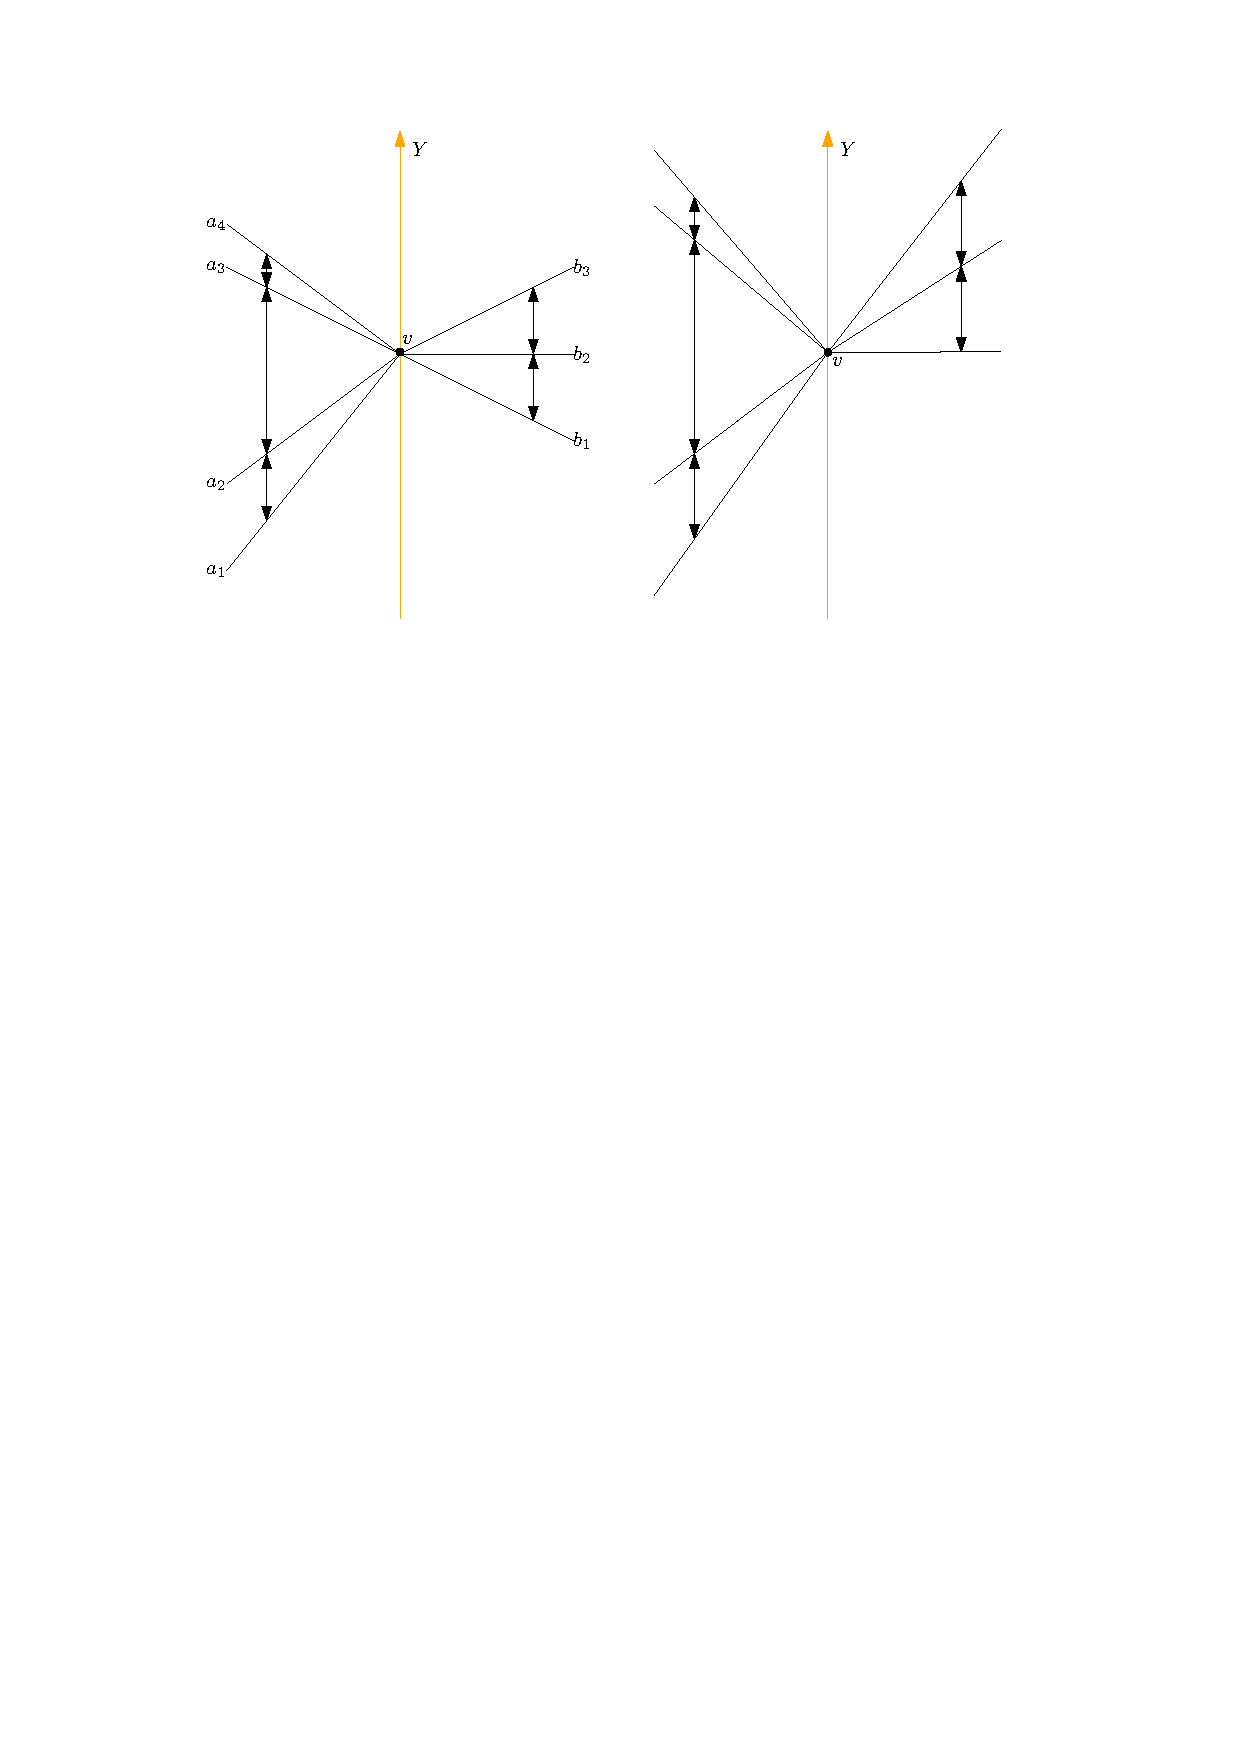
\includegraphics{figs/proportional}}
%	\caption{The degrees of freedom provided by the proportionality constraints}
%	\figlabel{proportional}
%\end{figure}
\begin{lem} \label{le:number-of-equations}
The total number of equations \thetag{\ref{eq:slope0}},~\thetag{\ref{eq:proportion}}, and~\thetag{\ref{eq:proportion2}} is $m-4$.
\end{lem} 

To achieve the desired number, $m$, of equations, we add
four \emph{boundary equations}.  If the outer face is a quadrilateral, we set
the slopes $s_1$, $s_a$, $s_b$, and $s_m$ of its edges $e_1$, $e_a$, $e_b$, and $e_m$ to the fixed values of the slopes of the edges of $\Delta$. If the outer face is a triangle $\alpha\beta\gamma$, with $\gamma\in Y$, we set the slopes $s_1$, $s_a$, and $s_m$ of the boundary edges $e_1$, $e_a$, and $e_m$ to the fixed values of the slopes of the edges of $\Delta$ and we pick another (non-boundary) edge $e_b$ incident to $\gamma$ and set its slope $s_b$ to a fixed value; this value is such that $s_b$ is either larger than each of $s_1$, $s_a$, and $s_m$ or smaller than each of $s_1$, $s_a$, and $s_m$, depending on whether the slope of $e_b$ in $G$ is larger than the slope of each of $e_1$, $e_a$, and $e_m$ or smaller than the slope of each of $e_1$, $e_a$, and $e_m$. Observe that no other cases are possible. Together with the proportionality constraints, this effectively pins all the slopes incident to $\gamma$ to fixed values.

Altogether, we have now a system of $m$ linear equations
in the $m$ unknowns $s=(s_1,\ldots,s_m)$, which we can write
compactly as
$A\cdot s = b$, with a square matrix $A$ whose entries come from
\thetag{\ref{eq:slope0}--\ref{eq:proportion2}}.
%are the variables we wish to solve for, and $b$ is a column $m$-vector
%whose entries also come from \eqref{slope}.  
Only four entries of
the right-hand side vector
$b$
are non-zero, due to the four boundary equations.
We will show that $A\cdot s=b$ has a unique
solution and that this solution gives a \Fary\ embedding of $G$.

\subsubsection{Setting Proportionality Constraints.}
%
%Since our plan is to show how to morph the given embedding of $G$ into the desired embedding, it is important that the given embedding satisfy the appropriate system of equations.  
%
We now specify how the coefficients in the proportionality constraints
are chosen, so that they are satisfied by the initial embedding.  The statement of \thmref{a-graph} assumes that $G$ is a \Fary\ embedding.  In this embedding, every edge $e$ intersects $Y$
in a single point $(0,y_e')$ and has a slope $s_e'$.  For a particular
vertex $v\in Y$, incident to edges $a_1,\ldots,a_k$ and $b_1,\ldots,b_\ell$
as described above, we use the slopes in the given embedding to set the
coefficients in the proportionality constraints.  In the notation used
in \eqref{proportion}, we set
$\lambda_i = (s_{b_i}'-s_{b_1}')/(s_{b_\ell}'-s_{b_1}')$
and in \eqref{proportion2}, we set $\mu = (s_{a_1}'-s_{a_k}')/(s_{b_\ell}'-s_{b_1}')$. This ensures that the slopes $s_{e_1}',\ldots,s_{e_m}'$ satisfy the
proportionality constraints.


\subsubsection{Ordering constraints.}
%
We define a relation $\prec$ on the edges of $G$, where $e_1 \prec e_2$ if and only if (1) $y_{e_1} < y_{e_2}$ and $e_1$ and $e_2$ have a common endpoint $v\in L$; or (2) $y_{e_1} > y_{e_2}$ and $e_1$ and $e_2$ have a common endpoint $v\in R$.
We say that a vector $s=(s_1,\ldots,s_m)$ \emph{satisfies the ordering
	constraints} if $s_{e_1} < s_{e_2}$ for every pair $e_1,e_2\in E(G)$
such that $e_1\prec e_2$. This definition captures the condition that vertices of $G$ in $L$ (respectively, $R$) should be embedded so that they remain in $L$ (respectively, $R$), as in the following. 

\begin{obs}\obslabel{left-right}
If a solution $s$ to $A\cdot s=b$ satisfies the ordering constraints, then every vertex that is in $L$ (in $R$) in $G$ is also in $L$ (respectively in $R$) in the embedding corresponding to $s$. 
\end{obs}

\begin{proof}	  
Consider any vertex $v$ that is in $L$ in $G$ and that is incident to (at least) two edges $e_1$ and $e_2$. Assume w.l.o.g.\ that $y_{e_1} < y_{e_2}$, and hence that $e_1 \prec e_2$. Since $s$ satisfies the ordering constraints we have $s_{e_1} < s_{e_2}$, hence the lines with slopes $s_{e_1}$ and $s_{e_2}$ through $(0,y_{e_1})$ and $(0,y_{e_2})$, respectively, meet in $L$. The argument for the vertices in $R$ is analogous. 
\end{proof}	  

Note that $\prec$ is acyclic since $G$ is an A-graph and therefore the slopes $s_{e_1}',\ldots,s_{e_m}'$ of edges
in $G$ satisfy the ordering constraints.  This would not be possible if $\prec$ contained cycles. 
%  Indeed, $i_1\prec
% \cdots \prec i_r$ implies that, for each $j\in\{3,\ldots,r\}$, $y_{i_j}\in
% (\min\{y_{i_{j-1}},y_{i_{j-2}}\}, \max\{y_{i_{j-1}},y_{i_{j-2}}\})$. Thus,
% a chain in $\prec$ corresponds to a sequence of strictly nested intervals.

\begin{lem}\lemlabel{order-gives-embedding}
	Any solution $s$ to $A\cdot s=b$ satisfying
	the ordering constraints % $\prec$
	yields a
	\Fary\ embedding of $G$.
\end{lem}

\begin{proofsketch}
Devillers \etal\ \cite{devillers.liotta.ea:checking} proved that a straight-line embedding $G'$ of a 2-connected graph $G$ is a \Fary\ embedding if: (i) for every vertex~$v$, the clockwise order of the edges around $v$ in $G'$ is the same as in $G$; and (ii) every face of $G$ is embedded without crossings in $G'$. In our case $G'$ is a straight-line embedding of $G$ given by a solution to $A\cdot s = b$ satisfying the ordering constraints. We prove that $G'$ satisfies conditions (i) and (ii) by using \obsref{left-right} and the fact that the slopes of the edges of $G'$ satisfy equations~\eqref{slope0}--(\ref{eq:proportion2}); in particular, for a vertex $v\in Y$, it is ruled out that the clockwise order of the edges around $v$ in $G'$ is reversed with respect to $G$ by the ordering constraints for the vertices of the triangles incident to $v$.
\end{proofsketch}


Any solution $s$ to $A\cdot s=b$ has the outer face drawn as $\Delta$, by the boundary constraints, and has the intersection between $e_i$ and $Y$ at $(0,y_i)$, by the concurrency constraints. Hence, by~\lemref{order-gives-embedding} ensuring the existence of a solution $s$ to $A\cdot s=b$ satisfying the ordering constraints is enough to prove~\thmref{a-graph}.

\subsubsection{Strong Ordering Constraints.}
\label{strong}
%
For some $\epsilon \ge 0$, we say that $s=(s_1,\ldots,s_m)$ satisfies
the \emph{$\epsilon$-strong ordering constraints} if, for each
$i,j\in\{1,\ldots,m\}$ such that $e_i\prec e_j$, the inequality
$s_j-s_i > \epsilon$ holds.
% A solution $s$ that satisfies
Clearly, any $s$ satisfying the $\epsilon$-strong ordering constraints also satisfies the ordering constraints. The converse holds when equations~\thetag{\ref{eq:slope0}}--\thetag{\ref{eq:proportion2}} are satisfied, for a suitably small $\epsilon$, as in the following.

\begin{lem}\lemlabel{weak-to-strong}
	Any solution $s$ to $A\cdot s=b$ that satisfies
	the ordering constraints
	also satisfies 
	the $\epsilon$-strong ordering constraints
	for all $\epsilon<\min\{|y_i-y_j| : 1\le i< j\le m\}$.
\end{lem}

\begin{proof}
	By \lemref{order-gives-embedding} every vertex is contained in the interior or on the boundary of $\Delta\subset[-1,1]^2$.
	Hence, every $x$-coordinate is
	in the interval $[-1,1]$.
	A vertex incident to $e_i$ and $e_j$ has $x$-coordinate
	$(y_j-y_i)/(s_i-s_j)$.
	From $|(y_j-y_i)/(s_i-s_j)|\le 1$ we derive
	$|s_i-s_j|\ge|y_j-y_i| > \epsilon$.
\end{proof}

\subsubsection{Uniqueness of Solutions Satisfying Ordering Constraints.}
%
The utility of the $\epsilon$-strong ordering constraints is that they
allow us to appeal to continuity. 
%It is impossible 
%to violate
%the ordering constraints without first violating the
%$\epsilon$-strong ordering constraints.
%But since the ordering constraints imply the
%$\epsilon$-strong ordering constraints,
%it is not possible
%to violate
%the ordering constraints at all.
% by showing that, if $A\cdot s=b$
%were to have some undesireable property, then some function which we
%know to be continuous would have a discontinuity.
An example will be seen in the following proof.

\begin{lem}\lemlabel{unique}
	If $s$ is a solution to $A\cdot s=b$ that satisfies the ordering
	constraints, % $\prec$, 
	then $s$ is 
	the unique solution to $A\cdot s=b$.
\end{lem}

\begin{proof}
	Assume that $\epsilon$ is fixed so that $0<\epsilon<\min\{|y_i-y_j| : 1\le i< j\le m\}$.
	
	Suppose, for a contradiction, that there is a solution $s$ to $A\cdot s=b$ that satisfies the ordering
	constraints, % $\prec$,
	but is not unique.  Since $A\cdot s=b$ is a linear system, there is an entire (at least) 1-parameter family of solutions,
	i.e., there is a non-zero $m$-vector $r$ such that, for every
	$\lambda\in\mathbb R$, $A(s+\lambda r)=b$.
	
	
	Define the continuous (in fact, piecewise linear) function $f(\lambda) := \min \{\, (s_j+\lambda r_j)-(s_i+\lambda r_i) : e_i \prec
	e_j\,\}$ and let $\lambda^*$ be the value with the smallest absolute value
	$|\lambda^*|$ such that
	$f(\lambda^*)\le\epsilon/2$. 
	
	In order to prove that $\lambda^*$ exists, it suffices to prove that a value $\lambda$ exists such that $f(\lambda)\le 0$. Note that $r_1=r_a=r_b=r_m=0$ since the slopes $s_1$, $s_a$, $s_b$, and $s_m$
	are fixed.
	Since $G$ is connected and $m\geq 5$, there is at least one vertex $v$ with two incident edges $e_k$
	and $e_\ell$ such that $r_k=0$ and $r_\ell\neq 0$. 
	We can thus pick $\lambda$ so that $(s_\ell+\lambda r_\ell)-(s_k+\lambda r_k)=s_\ell-s_k+\lambda r_\ell=0$,
	and then $f(\lambda)\le 0$. Hence $\lambda^*$ exists.
	
	Now we know that, for any $\lambda$ between $0$ and $\lambda^*$ and for any $i$ and $j$ such that $e_i\prec e_j$, the difference $(s_j+\lambda r_j)-(s_i+\lambda r_i)$ has the same sign as $s_j-s_i$. It follows that the slopes satisfy the ordering constraints throughout
	this interval, and
	\lemref{weak-to-strong} implies that $f(\lambda^*)\ge\epsilon$, a contradiction.
\end{proof}

%The proof of \lemref{unique} was quite explicit (perhaps overly so)
%in showing the discontinuity caused by the $\epsilon$-strong ordering
%constraints.  In subsequent arguments we will not be quite so explicit.

\subsubsection{A Parametric Family of Linear Systems.}
%
Note that $A$ and $b$ are functions of $y=(y_1,\ldots,y_m)$ and of the
four slopes $h=(s_1,s_a,s_b,s_m)$. We make this explicit, by writing
$A_1=A(y,h)$ and $b_1=b(y,h)$.

Let $y'=(y_1',\ldots,y_m')$ and $s'=(s_1',\ldots,s_m')$ denote the
$y$-intercepts and the slopes of the edges in the initial embedding of $G$
and let $h'=(s_1',s_a',s_b's_m')$. 

Consider the system $A(y',h')\cdot s = b(y',h')$.  This system has
at least one solution $s=s'$.  We now define
a continuous family of linear systems that interpolates between $A(y',h')\cdot s=b(y',h')$ and $A(y,h)\cdot s=b(y,h)$. Suppose first that the outer face of $G$ is delimited by a quadrilateral.

For $0\le t\le 1$ and $i\in\{1,a,b,m\}$,  define $s_i(t)=(1-t)s_i' + ts_i$ and $h(t)=(s_1(t),s_a(t),s_b(t),s_m(t))$.
Note that $s_1(t)-s_a(t) = (1-t)(s_1'-s_a') + t(s_1-s_a) > 0$. Inequalities $s_1'-s_a'>0$ and $s_1-s_a>0$ come from the assumption that the vertex incident to  $e_1$ and $e_m$ is in $L$ both in $G$ and in $\Delta$. Similarly, we have $s_m(t)-s_1(t)>0$ and $s_b(t)-s_m(t)>0$. Then we can define $\epsilon_1 = \min_{0\le t\le 1}\min\{s_1(t)-s_a(t), s_m(t)-s_1(t), s_b(t)-s_m(t)\}$ and observe that $\epsilon_1>0$. Analogously, for $0\le t\le 1$ and $i\in\{1,\ldots,m\}$, define $y_i(t) = (1-t)y_i' + ty_i$ and  $y(t)=(y_1(t),\ldots,y_m(t))$.
Note that, for any
$1\le i< j\le m$ and any $0\le t\le 1$, we have $y_j(t) - y_i(t) = (1-t)(y'_j-y'_i) + t(y_j-y_i) > 0$. Let $\epsilon_2=\min_{0\le t\le 1}\min\{y_j(t)-y_i(t): 1\le i< j\le m\}$ and observe that $\epsilon_2 >0$.  

  
%denominators in \eqref{slope} have absolute values bounded from below
%by $\epsilon_2$.  Thus, each entry in $A_t$ and $b_t$ is finite and is a
%uniformly continuous function of $t$.  

The entries in $A_t$ and $b_t$ are obtained in the same way as the entries of $A$ and $b$ were derived earlier, however each entry is now a linear function of~$t$, as $y$ and $h$ are replaced by $y(t)$ and $h(t)$, respectively, in the determination of the equations represented by $A_t$ and $b_t$.
Consider the unique quadrilateral $\Delta(t)$ whose edges cross $Y$ at
$y_1(t)$, $y_a(t)$, $y_b(t)$, $y_m(t)$ and have slopes $s_1(t)$,
$s_a(t)$, $s_b(t)$, and $s_m(t)$, respectively. Note that $\Delta(0)$ is the quadrilateral delimiting the outer face of $G$, while $\Delta(1)=\Delta$. Since $y_1(t),y_a(t),y_b(t),y_m(t)\in [-1,1]$, and since each of $s_1(t)$,
$s_a(t)$, $s_b(t)$, and $s_m(t)$ is at least $\epsilon_1$, we have that $\Delta(t)\subset[-1/\epsilon_1,1/\epsilon_1]\times[-\infty,\infty]$.
Hence, after scaling the $x$-coordinates by $1/\epsilon_1$,
\lemref{weak-to-strong} applies to $A_t\cdot s =b_t$, so any solution $s$
that satisfies $\prec$ also satisfies the $\epsilon^*$-strong ordering
constraints, for $\epsilon^*=\epsilon_1\cdot\epsilon_2$.

If the outer face of $G$ is delimited by a triangle, the arguments are analogous, however the inequalities $s_1(t)-s_a(t)>0$ and $s_m(t)-s_1(t)>0$ become either $s_m(t)-s_1(t)>0$ and $s_a(t)-s_m(t)>0$ or $s_1(t)-s_m(t)>0$ and $s_a(t)-s_1(t)>0$, depending on whether $(0,y_1)$ or $(0,y_m)$ is a vertex of $G$, respectively. Further, the inequality involving $s_b(t)$ now states  either $s_b(t)-s_a(t)>0$ or that $s_b(t)$ is smaller than the smallest between $s_1(t)$ and $s_m(t)$, depending on which of the two holds in $G$ (as when determining the boundary equations).

\subsubsection{Existence (and uniqueness) of solutions to $A_t\cdot s=b_t$.}
%
We now prove the following lemma which, together with \lemref{order-gives-embedding}, completes the proof of \thmref{a-graph}.

\begin{lem}\lemlabel{uniqueness}
	For every $0\le t\le 1$, the system $A_t\cdot s=b_t$ has a unique solution,
	and this solution satisfies the ordering constraints. % $\prec$.
\end{lem}

\begin{proof}
	Since $A_t$ is an $m\times m$ matrix, the system $A_t\cdot
	s=b_t$ has a unique solution~$s$ if and only if $\det A_t \neq 0$.
	When $\det A_t =0$, the system may have no solutions or
	multiple solutions.  
	When $\det A_t\neq 0$, 
	Cramer's Rule states that
	the solution
	is $s(t)=(s_1(t),\ldots,s_m(t))$ where, for each
	$i\in\{1,\ldots,m\}$, $s_i(t) = \frac{\det A_t^i}{\det A_t }$,
	and $A_t^i$ denotes the matrix $A_t$ with its $i$-th column replaced
	by $b_t$. 
	The numerators $\det A_t^i$ and the common
	denominator $\det A_t $ are polynomials in $t$, and therefore
	continuous
	functions of $t$.
	The solution $s(t)=(s_1(t),\ldots,s_m(t))$ depends continuously on $t$
	as long as  $\det A_t\ne0 $.
	
	
	We know that $A_0\cdot s=b_0$ has a solution $s'$ that satisfies the ordering constraints. By \lemref{unique}, this solution is unique, so $\det A_0\neq 0$.
	%
	Let $t^*:=\min \{t>0 :\det A_{t}= 0\}$. If $t^*$ does not exist we set $t^*=\infty$.
	% or $t>1$, we are
	% done.
	
	First we argue that, for $0\le t <\min \{1,t^*\}$, the unique solution $s(t)$ to $A_t\cdot s=b_t$ satisfies the ordering constraints. This argument is similar to the proof of \lemref{unique}. Suppose, for a contradiction, that a value $0<t<\min\{1,t^*\}$ exists for which $s(t)$ does not satisfy the ordering constraints. As $t$ increases its value from $0$ to $\min\{1,t^*\}$, since $s(t)$ depends continuously on $t$, a value is reached in which $s(t)$ violates the $\epsilon^*$-strong ordering constraints, while it does not violate the ordering constraints. This contradicts	\lemref{weak-to-strong}.
	
	If $t^*>1$ the same argument applies to $t=1$ and we are done.
	Assume, for a contradiction, that $0<t^*\le 1$.
	We look at whether the limit $s^*=\lim_{t\uparrow t^*}
	s(t)$ exists.
	Each function $s_i(t)$ is a quotient of two polynomials; thus, for $t\to t^*$ it can either converge to $s_i(t^*)$ continuously, or diverge to $+\infty$ or $-\infty$.
	%
	For $t<t^*$ all solutions $s(t)$ to the systems $A_t\cdot s=b_t$ satisfy the $\epsilon^*$-strong ordering constraints.
	Hence, if the limit exists, by continuity, it also satisfies $A_{t^*}\cdot s^*=b_{t^*}$
	and the $\epsilon^*$-strong ordering constraints.
	By \lemref{unique}, the solution $s^*$ is
	the unique solution
	of $A_{t^*}\cdot s=b_{t^*}$, which contradicts the assumption
	$\det A_{t^*}= 0$.
	
	The proof of the lemma is completed by ruling out the possibility that $A_{t^*}\cdot s=b_{t^*}$ has no solution because $\lim_{t\uparrow t^*} s(t)$ does not exist. This proof is deferred to the full version of the paper in the appendix. 
\end{proof}

%!TEX root = mainShort.tex
\section{Triangulations}
\seclabel{triangulations}

%We will sometimes make use of this simple fact:
%\begin{obs}\obslabel{quad}
%	If $q=abcd$ is a simple quadrilateral, then neither of the segments $ac$
%	or $bd$ cross any of the edges of $q$.
%\end{obs}

%As is the case with \thmref{a-graph} there is an annoying case distinction
%that occurs when $Y$ contains vertices on the outer face.  

In this section we prove that every collinear set is free. Recall that a {\em triangulation} is a (not necessarily straight-line) plane embedding of an edge-maximal planar graph. Let $T$ be a triangulation, let $r_1,\ldots,r_k$ be a sequence of vertices and edges in $T$, and let $y_1<\cdots<y_k$ be a sequence of numbers. A triangle $\Delta=\alpha\beta\gamma$ is \emph{compatible} with $r_1,\ldots,r_k$ and $y_1,\ldots,y_k$ if the following conditions hold: (1) if $r_1$ is a vertex, then $\beta=(0,y_1)$, otherwise $(0, y_1)$ in the interior of the edge $r_1=\beta\gamma$; and (2) if $r_m$ is a vertex, then $\alpha=(0,y_m)$, otherwise $(0,y_m)$ in the interior of the edge $r_m=\alpha\gamma$. We have the following.


%A triangulation is \emph{admissible} if the intersection of $Y$ with each edge of the triangulation is either empty, a single point,
%or the entire edge.  


\begin{thm}\thmlabel{main}
	Let $T$ be a triangulation and $C$ be an admissible curve for $T$. Further, let $y_1<\cdots<y_k$ be a sequence of numbers and let $r_1,\ldots,r_k$ be the sequence of vertices and open edges of $T$ that are intersected by $C$, in the order in which they are intersected by $C$ (each edge of $T$ that is entirely on $C$ has its end-vertices represented by two consecutive elements $r_i$ and $r_{i+1}$ of $r_1,\ldots,r_k$, while the open edge is not in $r_1,\ldots,r_k$). Finally, let $\Delta$ be a triangle that is compatible with 
		$r_1,\ldots,r_k$ and $y_1,\ldots,y_k$.

	Then, for any $\epsilon>0$, $T$ has a \Fary\ embedding such that the outer face is delimited by $\Delta$ and such that the following hold for each $i=1,\ldots,k$: (1) if $r_i$ is a vertex, then it is drawn at $(0,y_i)$; and (2) if $r_i$ is an edge, then the intersection of $r_i$ with $Y$ has $y$-coordinate in the interval $[y_i-\epsilon,y_i+\epsilon]$.
\end{thm}

\begin{proof}
	%   We call $y_i$ the (desired) \emph{crossing coordinate} for $r_i$. If
	%   a \Fary\ embedding contains an edge whose intersection with the
	%   $y$-axis is $\{(0,y)\}$ or a vertex at $(0,y)$, we say that the edge
	%   or vertex \emph{crosses the $y$-axis at $y$}.
	%
	%   Let $L=C^-$, $R=C^+$.  
We start by classifying the edges of $T$. An edge of $T$ is \emph{marked} if its intersection with $C$ is non-empty, otherwise it is \emph{unmarked}. A marked edge might intersect $C$ in a single point (then it is a \emph{crossing edge}), or might lie on $C$. If an edge lies on $C$ or if it is unmarked, then it is a \emph{non-crossing edge}. 
	
	%   We prove an extension of the theorem to the case where $T$ is an
	%   non-crossing embedded graph whose faces consist of triangles (3-cycles)
	%   and quadrilateral (4-cycles) with the resriction that, for every
	%   quadrilateral face $q$, all four edges of $q$ are crossing edges.
	%   The proof is by induction on the number of non-crossing edges plus the
	%   number of vertices of $T$.
	
	%   \paragraph{Base Cases:}
	%   There are three base cases tht we handle explicitly.  If $T$ contains
	%   2 or fewer crossing edges, If $T$ is the complete graph, $K_4$ on 4
	%   vertices, but only has only three crossing edges, then the theorem is
	%   also easy to prove directly.  The last base case occurs when all edges
	%   of $T$ are crossing edges.  In this case $T$ is bipartite and therefore
	%   all its faces are quadrilaterals, so $T$ is a quadrilateralization.
	%   This case is handled directly by \lemref{quad2}.
	%
	%   Thus we may assume that $T$ has at least one non-crossing edge and
	%   at least 2 crossing edges.  
	
	The proof is by induction on the number of vertices of $T$, primarily, and on the number of non-crossing edges of $T$, secondarily.
	We begin by describing reductions that allow us to apply the
	inductive hypothesis. When none of these reductions applies,
	we arrive at our base case. To handle the base case 
	we remove every unmarked edge of $T$ to obtain an A-graph, on which we
	apply \thmref{a-graph}.

% we argue that
%	$T$ has a sufficiently simple structure that it can be handled by
%	\thmref{a-graph}.  In particular, when no reduction applies, we can
	
%	Before continuing, we dispense with one easy special case.  If $Y$
%	contains an edge $e$ of the outer face, then every vertex
%	of $G$ is contained in $L\cup Y$ or every vertex of $G$ is contained
%	in $Y\cup R$.  In this case, the definition of compatible triangle
%	implies that the edge $\alpha\beta$ of $\Delta$ is contained in the
%	$y$-axis.  In this case, we can simply apply Tutte's Convex Embedding
%	Theorem to obtain a \Fary\ embedding of $G$ in which the outer face is embedded
%	on $\Delta$ with $e$ embedded on $\alpha\beta$, .  This embedding
%	satisifies all the conditions of the theorem.  Therefore, for the
%	remainder of this proof, we assume that $C$ intersects the interior
%	of at least one inner face of $T$.
	
	\subsubsection{Separating Triangles.}
	%(See \figref{separating}.)
	If $T$ contains a separating triangle $xyz$, then denote by $T^+$ (respectively, $T^-$) the triangulation obtained from $T$ by removing all the vertices in the interior (respectively, exterior) of $xyz$. Note that $xyz$ delimits an inner face of $T^+$ and the outer face of $T^-$. 
	
	If the interior of $xyz$ does not intersect $C$, we apply induction on $T^+$ (note that $|V(T^+)|<|V(T)|$) and then use Tutte's Convex Embedding Theorem  \cite{tutte:how} to draw $T^-$ so that its outer face is delimited by the triangle representing the cycle $xyz$ in the constructed \Fary\ embedding of $T^+$.
	
%	\begin{figure}[tb]
%		\centering{\includegraphics{figs/separating}}
%		\caption{Recursing on separating triangles in the proof of
%			\thmref{main}}
%		\figlabel{separating}
%	\end{figure}
	If the interior of $xyz$ intersects $C$, then the vertices and edges of $T$ intersected by $C$ that are not in $T^+$ form a contiguous
	subsequence $r_i,\ldots,r_j$ of $r_1,\ldots,r_k$. Each of $r_{i-1}$ and $r_{j+1}$ is either an edge or a vertex of $xyz$.  
	Let $\epsilon'$ be any
	value less than $\min\{\epsilon,y_{i}-y_{i-1}, y_{j+1}-y_j\}$. Apply induction on $T^+$ with value $\epsilon'$ and sequences $r_1,\ldots,r_{i-1},r_{j+1},\ldots,r_k$ and
	$y_1,\ldots,y_{i-1},y_{j+1},\ldots,y_k$. In the obtained \Fary\ embedding of $T^+$ let $\Delta'$ be the triangle representing  $xyz$ and let $y_{i-1}'$ and $y_{j+1}'$
	be the $y$-coordinates of the intersections of
	$r_{i-1}$ and $r_{j+1}$ with $Y$.  By the choice of
	$\epsilon'$ we have $y_{i-1}'<y_i<\cdots<y_j<y_{j+1}'$.  Observe that
	$\Delta'$ is compatible with $r_{i-1},\ldots,r_{j+1}$ and
	$y_{i-1}',y_i,\ldots,y_j,y_{j+1}'$.
	%
	Apply induction on $T^-$ with value $\epsilon$ using the triangle $\Delta'$ and the sequences $r_{i-1},\ldots,r_{j+1}$ and
	$y_{i-1}',y_i,\ldots,y_{j},y_{j+1}'$.  Combining the \Fary\ embeddings of $T^+$
	and $T^-$ yields the desired \Fary\ embedding of $T$. In the following we assume that $T$ has no separating triangles.
	
	
	\begin{figure}[tb]
		\centering{\includegraphics[scale=0.85]{figs/contractible}}
		\caption{Contracting and uncontracting edges in the proof of
			\thmref{main}}
		\figlabel{contractible}
	\end{figure}

	\subsubsection{Contractible Edges.}
	(See \figref{contractible}.)
	A face of $T$ is a \emph{crossing
		face} if it is incident to two crossing edges.  An
	unmarked edge of $T$ is \emph{contractible} if it is not contained
	in the boundary of any crossing face.  
	
	If $T$ contains a contractible edge $xy$ then we contract $xy$ to
	obtain a new vertex $v$ in a smaller triangulation $T'$.   We then apply
	induction on $T'$ with the value $\epsilon'=\epsilon/2$ to obtain a \Fary\
	embedding of $T'$ such that each crossing edge $e_i$ crosses
	$Y$ in the interval $[y_i-\epsilon/2,y_i+\epsilon/2]$.
	%
	To obtain a \Fary\ embedding of $T$ we uncontract $v$ by placing $x$ and $y$
	within a ball of radius $\epsilon/2$ centered at $v$. (That such
	a placement is always possible is a standard argument, see, e.g.,~\cite{fary,w-sp-05}.)  Since the
	distance between $y$ and $v$ and the distance between $x$ and $v$ are each at most $\epsilon/2$,
	each crossing edge $r_i$ incident to $x$ or $y$ crosses $Y$ in the interval $[y_i-\epsilon,y_i+\epsilon]$, as required.
	From now on we assume that $T$ has no separating triangles or contractible
	edges.
	
	%   \paragraph{Eraseable edges}
	%   We say that a non-crossing edge of $xy$ of $T$ is \emph{eraseable}
	%   if neither of its endpoints is on $C$ and both its incident faces
	%   intersect $C$.  If $T$ contains an eraseable edge $xy$, then we remove
	%   the edge $xy$ from $T$ to obtain smaller graph $T'$ on which we can
	%   apply induction. In the resulting drawing of $T'$, $x$ and $y$ lie on
	%   a common face (which may be the outer face of $T'$) and are visible.
	%   We can therefore add the edge $xy$ to obtain the desired drawing
	%   of $T$.
	
	\subsubsection{Flippable edges.} (See \figref{flippable}.) We say that an unmarked edge $xy$ of $T$ is \emph{flippable} if there
	exist distinct vertices $z$, $a$, $b$, and $c$ such that: (1) $xyb$, $zyc$, $xza$ are crossing faces of $T$; (2) $xyz$ is a non-crossing face of $T$; and either (3a) $C$ intersects $za$, $xa$, $xb$, $yb$, $yc$, and $zc$ in this order, or (3b) $C$ intersects $xa$, $xb$, $yb$, $yc$, $zc$, and $za$ in this order.  
	
	If $T$ contains the flippable edge $xy$ then we replace it with $zb$ to obtain a new triangulation $T'$. Note that, since $T$ has no separating triangles, the edge $zb$ is not in $T$. Further, $T'$ has the same number of vertices of $T$ and one less non-crossing edge. After choosing a crossing coordinate $y_{zb}$ for $zb$ between those $y_{xb}$ and $y_{yb}$ of $xb$ and $yb$, respectively, we can inductively embed $T'$ with value $\epsilon$ and sequences $r_1,\dots,xb,zb,yb,\dots,r_k$ and $y_1,\dots,y_{xb},y_{zb},y_{yb},\dots,y_k$.
	%
	We claim that in the resulting \Fary\ embedding of $T'$, the only open edge
	that intersects the open segment $xy$ is $zb$. It suffices to prove that $z$ is not a reflex vertex in the quadrilateral $xbyz$; note that $b$ is not a reflex vertex in $xbyz$, since $bx$ and $by$ are crossing edges. In Case~(3a), the existence of the
	edges $za$ and $zc$ ensures that, in the \Fary\ embedding of $T'$,
	$xbyz$ is convex. In Case~(3b), the triangle $zxa$ is convex and $xbyz$ is contained in this triangle, therefore $z$ is convex. In either case, removing $zb$ from the \Fary\ embedding of $T'$ and replacing it with $xy$ yields the desired \Fary\ embedding of $T$.
	
	\begin{figure}[tb]
		\centering{\includegraphics[scale=0.85]{figs/flippable}}
		\caption{Flipping edges in the proof of
			\thmref{main}}
		\figlabel{flippable}
	\end{figure}
	
	
	\subsubsection{Edges on $C$.} If $T$ contains an edge $xy$ that lies on $C$, then we treat it as we treated flippable edges. In this case, $xy$ is incident to two triangles $xyz$ and $yxb$ with $z\in C^+$ and $b\in C^-$. We replace $xy$ with an edge $zb$ to obtain a new triangulation $T'$ with the same number of vertices of $T$ and one less non-crossing edge. We apply induction and get a \Fary\ embedding of $T'$, in which $z$ and $b$ are
	on opposite sides of $Y$ and $x$ and $y$ are on $Y$, hence 	neither $z$ nor $b$ is a reflex vertex of the quadrilateral $xzyb$.
	Thus, removing $zb$ and adding $xy$ gives a \Fary\ embedding of $T$.
	
	\subsubsection{Base case.} We are left with the case in which $T$ is a triangulation
	with no separating triangles, no contractible edges, no flippable
	edges, and no edge contained in $C$.  If $T$ is the complete graph
	on three or four vertices, then the proof is trivial,
	so we may assume that $T$ has at least 5 vertices.
	
	\begin{claimx} \obslabel{unmarked}
	Any unmarked edge $xy \in C^+$ is on the boundary of two faces $xyz$ and $yxb$ where $z,b\in\{C \cup C^-\}$.
	\end{claimx}

	Symmetrically, every unmarked edge $xy\in C^-$ is incident to two faces
	$xyz$ and $yxb$ with $z,b\in \{C \cup C^+\}$.  This implies that no face of $T$ contains more than one unmarked edge.
	%
	Thus, every unmarked edge of $T$ is incident to two faces that intersect $C$. The union of these two faces is a quadrilateral whose boundary consists of four edges that intersect $C$.
	Let $\tilde{G}$ denote the embedded plane graph obtained by removing all unmarked edges
	from $T$.  By \thmref{dujmovic-frati}, we know that $\tilde G$ has
	a \Fary\ embedding $G$ whose edges and vertices intersect $Y$ in the
	same order as the same edges and vertices intersect $C$ in $\tilde{G}$. We have the following.
	
	\begin{claimx} \label{claim-a-graph}
		$G$ is an A-graph.
	\end{claimx}
	
	%
	%The graph $Q^*$ has two triangular faces $vab$
	%   and $vcd$ incident to $v$ such that $ab=r_{i-1}$ and $cd=r_{i+1}$.
	%   Split $v$ into two vertices $x\in L$ and $y\in R$ joined by the edge
	%   $xy$, make $x$ adjacent to all neighbours of $v$ in $R$, and make
	%   $y$ adjacent to all neighbours of $v$ in $L$. See \figref{split}.
	%   This splitting operation eliminates the triangular faces $vab$ and
	%   $vcd$ and introduces the quadrangular faces $xyab$ and $yxcd$.
	%
	%   \begin{figure}
	%      \centering{
	%        \begin{tabular}{c|c}
	%            \includegraphics{figs/split} & \includegraphics{figs/split-outer}
	%        \end{tabular}}
	%      \caption{Splitting vertices on $C$ in the proof of
	%      \thmref{main}.}
	%      \figlabel{split}
	%   \end{figure}

	We can hence apply \thmref{a-graph} to
	obtain a \Fary\ embedding of $G$ in which the intersection of $r_i$
	with $Y$ is at $(0,y_i)$.  Each internal edge $ac$ of $T$ not in $G$
	corresponds to a quadrangular face $q=abcd$ of $G$ in which $a$ or $c$ is a
	reflex vertex.  Therefore, the edge $ac$ can be added to the embedding
	without introducing crossings.  A single external edge $\alpha\beta$
	on the outer face of $T$ might not appear in $G$. In this case the outer
	face of $G$ is a quadrilateral $q'=\alpha a \beta b$ in which $a$ or $b$ is
	a reflex vertex, so the segment $\alpha\beta$ lies outside of $q'$, and the edge $\alpha\beta$ can therefore be added to the embedding of $G$
	without introducing crossings. Reinserting each edge of $T$ not in $G$ gives the desired
	\Fary\ embedding of $T$. This concludes the proof of \thmref{main}.
\end{proof}
	
We are finally ready to prove \thmref{our-bang}. Given an embedded plane graph $G$, a collinear set $S$ in $G$,
	and any $y_1'<\cdots<y_{|S|}'$, we need to prove that $G$ has
	a \Fary\ embedding in which the vertices in $S$ are embedded at
	$(0,y_1'),\ldots,(0,y_{|S|}')$. We can assume that $G$ is a triangulation. Indeed, if it is not,  edges can be added to it so that it becomes a triangulation, while preserving the property that $S$ is collinear set; after constructing a \Fary\ embedding in which the vertices of $S$ are embedded at $(0,y_1'),\ldots,(0,y_{|S|}')$ the inserted edges can be removed obtaining the desired \Fary\ embedding of the initial graph. Assume hence that $G$ is a triangulation. 	 \thmref{dujmovic-frati} implies
	that there exists a Jordan curve $C$ that is admissible for $G$
	and that contains all the vertices of $S$ in some order, say
	$v_1,\ldots,v_{|S|}$.  The curve $C$ intersects a subset of the edges
	and vertices of $G$ in some order $r_1,\ldots,r_k$.  We choose any
	sequence $y_1<\cdots<y_k$ so that, for all $i\in\{1,\ldots,k\}$ and
	$j\in\{1,\ldots,|S|\}$, $y_i = y_j'$ if $r_i=v_j$.  We select
	any triangle $\Delta$ that is compatible with $r_1,\ldots,r_k$ and
	$y_1,\ldots,y_k$ and choose $\epsilon = \min\{(1/3)(y_{i+1}-y_{i}):
	i\in\{1,\ldots,k-1\}\}$.  \thmref{main} then gives us a \Fary\
	embedding of $G$ in which the vertices in $S$ are embedded at $(0,y_1'),\ldots,(0,y_{|S|}')$, as required by \thmref{our-bang}.











\section{Concluding Problems}

In this paper we proved that every collinear set is a free set. Several problems concerning collinear and free sets remain open. Here we mention our favorite two.

Let $f(n)$ be the minimum, over all $n$-vertex planar graphs $G$, of the size of the largest collinear set in $G$. What is the growth rate of $f(n)$? The best known bounds are $f(n)\in\Omega(\sqrt{n})$ and $f(n)\in \mathcal{O}(n^\sigma)$, for $\sigma < 0.986$ \cite{bose.dujmovic.ea:polynomial,ravsky.verbitsky:on}. Our results prove that $f(n)$ is also the minimum size of the largest free set over all $n$-vertex planar graphs; this makes determining the growth rate of $f(n)$ even more relevant.
%
%\begin{op}
%	What is the growth rate of $f(n)$?
%\end{op}

We find interesting to understand whether our main theorem can be generalized so that the $y$-coordinates are arbitrarily prescribed not only for the vertices on $Y$, but also for the crossing points of the edges with $Y$. Note that \thmref{main} {\em almost} gives this generalization, as every edge crossing $Y$ is at most $\epsilon$ away from its prescribed crossing point, for any arbitrarily small $\epsilon$. 

%\section*{Acknowledgement}
%
%Part of this research was conducted during the 5\textsuperscript{th} and the 6\textsuperscript{th} Workshops on Geometry and Graphs, held at the Bellairs Research Institute, March 5--10, 2017 and March 11--16, 2018.  We are grateful to the organizers and participants for providing a stimulating research environment.
%
%This work was initiated at the \emph{Fifth Workshop on Geometry and
%	Graphs}, held at the Bellairs Research Institute, March 5--10, 2017 and
%was picked up again at the \emph{Sixth Workshop on Geometry and Graphs},
%March 11--16, 2018.  We are grateful to the organizers and the other
%workshop participants for providing a stimulating research environment.

\newpage
\bibliographystyle{plain}
\bibliography{freecoll}

\end{document}









